% !TeX root = Steiger_Miro_Abschlussarbeit.tex
\documentclass[a4paper,11pt]{article} %Schriftgröße
\usepackage[T1]{fontenc} 
\usepackage[utf8]{inputenc}
\usepackage{csquotes}
\usepackage{listings}
\usepackage[ngerman]{babel}%Veröffentlichungssprache
\usepackage{graphicx}
\usepackage{amsmath}
\usepackage{textgreek}
\usepackage[export]{adjustbox}
\usepackage{ragged2e}
\usepackage[format=plain,justification=RaggedRight,singlelinecheck=false,font={small},labelsep=colon]{caption}
\usepackage{xcolor}	
\usepackage{makecell}
\usepackage{algorithm} 
\usepackage{algpseudocode} 
\usepackage[a4paper]{geometry}
\geometry{left=2.62cm,right=3.28cm,top=2cm,bottom=2.4cm}%Seitenränder
\usepackage[onehalfspacing]{setspace}%Zeilenabstand
\renewcommand{\\}{\vspace*{0.5\baselineskip} \newline}
\renewcommand*\MakeUppercase[1]{#1}	
\usepackage{fancyhdr}
\pagestyle{fancy}
\renewcommand{\headrulewidth}{0pt}
\renewcommand{\footrulewidth}{0pt}
\renewcommand{\familydefault}{\sfdefault}
\fancyhead[R]{\footnotesize{\thepage}}
\fancyhead[L]{\footnotesize{\leftmark}}
\fancyfoot{}


%%Font Size für Kapitel-Überschriften
\usepackage{titlesec}

\titleformat*{\section}{\LARGE\bfseries\sffamily}
\titleformat*{\subsection}{\Large\bfseries\sffamily}
\titleformat*{\subsubsection}{\large\bfseries\sffamily}

\usepackage{etoolbox}
\usepackage[colorlinks,
pdfpagelabels,
pdfstartview = FitH,
bookmarksopen = true,
bookmarksnumbered = true,
linkcolor = black,
urlcolor = black,
plainpages = false,
hypertexnames = false,
citecolor = black]{hyperref}
\usepackage[parfill]{parskip}


%scalebox für formeln
\newcommand*{\Scale}[2][4]{\scalebox{#1}{$#2$}}%


%%rename "Chapter" to "Kapitel"
\addto\extrasngerman{\def
\sectionautorefname{Kapitel}
} %Definition "Kapitel" bei autoref von section

\addto\extrasngerman{\def
\subsectionautorefname{Kapitel}
} %Definition "Kapitel" bei autoref von subsection

\addto\extrasngerman{\def
\subsubsectionautorefname{Kapitel}
} %Definition "Kapitel" bei autoref von subsubsection

% Harvard Citation style
\usepackage[style=authoryear-comp, backend=biber, maxnames=2, maxbibnames=99]{biblatex}

\DefineBibliographyStrings{ngerman}{
   andothers = {{et\,al\adddot}},
}


%biblatex-config
\makeatletter
\newrobustcmd*{\parentexttrack}[1]{%
  \begingroup
  \blx@blxinit
  \blx@setsfcodes
  \blx@bibopenparen#1\blx@bibcloseparen
  \endgroup}

\AtEveryCite{%
  \let\parentext=\parentexttrack%
  \let\bibopenparen=\bibopenbracket%
  \let\bibcloseparen=\bibclosebracket}

\makeatother
\renewcommand*{\nameyeardelim}{\addcomma\space}
\addbibresource{chapters/literature/refs.bib}


\begin{document}
\numberwithin{equation}{section}

%%%%%%%%%%%%%%%%%%%%%%%%%%%%%%%%
%%%%%%%%%% TITELSEITE %%%%%%%%%%
%%%%%%%%%%%%%%%%%%%%%%%%%%%%%%%%
\begin{titlepage}
	\begin{flushleft}
		
\includegraphics[width=\textwidth]{Grafiken/TH/TH.png}\\
		\vspace*{2cm}
	\end{flushleft}

	\begin{flushleft}
		Bachelorarbeit Medientechnologie
	\end{flushleft}

	\begin{huge}
		\noindent
		\bfseries
		Effizientes und realistisches Partikelsystem zur Simulation von Feuer und Rauch in VR-Umgebung \\
	\end{huge}
	~\\
	~\\
	\noindent
	vorgelegt von                   \\
	\textbf{Miro Steiger}			\\
	~\\
	~\\
	\noindent
	Erstgutachter: Prof. Dr.-Ing. Arnulph Fuhrmann (Technische Hochschule Köln)              \\
	Zweitgutachter:  Prof. Dr. rer. nat. Stefan Michael Grünvogel (Technische Hochschule Köln)
	~\\
	~\\
	Köln, 28.07.2022
	~\\
	~\\
	\begin{figure}[b]
		\begin{flushright}
			
\includegraphics[scale=1]{Grafiken/TH/TH_F07_cover.png}\\
		\end{flushright}
	\end{figure}

	\pagenumbering{Roman}
	\pagestyle{fancy}
\end{titlepage}



%%%%%%%%%%%%%%%%%%%%%%%%%%%%%%
%%%%%%%%%% ABSTRACT %%%%%%%%%%
%%%%%%%%%%%%%%%%%%%%%%%%%%%%%%
\newpage

\markboth{Bachelorarbeit}{Bachelorarbeit}
\addtocounter{page}{1}

\begin{flushleft}
	\begin{huge}
		\textbf{Bachelorarbeit}
	\end{huge}
	~\\
	~\\
	\textbf{Titel:}  Effizientes und realistisches Partikelsystem zur Simulation von Feuer und Rauch in VR-Umgebung
	~\\
	\doublespacing
	\textbf{Gutachter:}
	\begin{description}
		\vspace{-0.2cm}
		\itemsep-8pt
		\item[–]
			Prof. Dr. Arnulph Fuhrmann (TH Köln)
		\item[–]
			Prof. Dr. rer. nat. Stefan Michael Grünvogel (TH Köln)
	\end{description}
	\vspace{-0.4cm}
	\singlespacing
	\textbf{Zusammenfassung:} Der Einsatz von Virtual Reality findet in immer mehr Bereichen
	seinen Nutzen. Im Bereich der Brandbekämpfung könnte die Technik eine sichere und
	kostengünstigere Alternative zu bestehenden Trainingsmethoden sein.
	Aktuelle Anwendungen legen bisher jedoch nicht viel Wert auf wirklich immersive Erfahrungen
	beim Rendering der Brände. Durch realistischere Renderings kann der Nutzer in echte Stresssituationen
	versetzt werden. Parallax Occlusion Mapping und Raymarching sind zwei Methoden, welche sich für die
	Darstellung von Feuer und Rauch in virtueller Realität anbieten.
	In dieser Arbeit werden daher die beiden vorgeschlagenen Algorithmen in einem Partikelsystem implementiert, verglichen und
	hinsichtlich ihrer Performance, optischer Qualität und den Einsatzmöglichkeiten in einem Brandsimulator bewertet.
	\singlespacing
	\textbf{Stichwörter:} Virtual Reality, Partikelsystem, Parallax Occlusion Mapping, Volumen Rendering, Raymarching, Echtzeitrendering\\
	\doublespacing
	\textbf{Datum:} 28.07.2022


	\vspace{1cm}

	\begin{huge}
		\textbf{Bachelors Thesis}
	\end{huge}
	~\\
	% ~\\
	\textbf{Title:} Efficient and realistic particle system to render fire and smoke in VR
	~\\
	\doublespacing
	\textbf{Reviewers:}
	\begin{description}
		\vspace{-0.2cm}
		\itemsep-8pt
		\item[–]
			Prof. Dr. Arnulph Fuhrmann (TH Köln)
		\item[–]
			Prof. Dr. rer. nat. Stefan Michael Grünvogel (TH Köln)
	\end{description}
	\vspace{-0.4cm}
	\singlespacing
	\textbf{Abstract:}
	The use of virtual reality extends into more and more areas.
	In the field of firefighting, the technique could be a safe and cheaper
	alternative to existing fire training methods.
	However, current applications focused less on truly immersive experiences when it
	comes to the rendering the fires. More realistic renderings can put the user in higher
	stressful situations.
	Parallax occlusion mapping and raymarching are two methods that are suitable
	for displaying fire and smoke in a stereoscopic view.
	In this thesis, the two proposed algorithms are implemented in a particle system, compared and
	evaluated with regard to their performance, appearance and possible uses in a fire simulator.
	\singlespacing
	\textbf{Keywords:} Virtual Reality, Particle System, Parallax Occlusion Mapping, Volume Rendering, Raymarching, Real Time Rendering\\
	\doublespacing
	\textbf{Date:} 28.07.2022
\end{flushleft}

% - Im Abstract weniger blabla \\ done
% - Beschreiben, womit das Partikelsystem erzeugt wird\\ done
% - Warum ?\\ done
% - Was wird in dieser Arbeit überhaupt gemacht? -> Vergleich Parallax Mapping / Raymarching done

\newpage


%%%%%%%%%%%%%%%%%%%%%%%%%%%%%%
%%%%%%%%%%  INHALT  %%%%%%%%%%
%%%%%%%%%%%%%%%%%%%%%%%%%%%%%%

\renewcommand*\contentsname{Inhalt}
\vspace{3cm}
\tableofcontents
\newpage
\pagenumbering{arabic}


%%%%%%%%%%%%%%%%%%%%%%%%%%%%%%
%%%%%%%%%%  KAPITEL %%%%%%%%%%
%%%%%%%%%%%%%%%%%%%%%%%%%%%%%%
\section{Einleitung}
\markboth{Einleitung}{Einleitung}
\noindent

Die Simulation von Feuer und Rauch ist ein viel diskutiertes Thema in der Computergrafik. Einerseits
spielen diese besonders in Videospielen und Filmproduktionen eine außerordentlich große Rolle. Auf der
anderen Seite helfen solche Simulationen auch im Bereich der Gefahrenbekämpfung und -vorbeugung.
So kann eine realistische Feuersimulation dazu beitragen, einen Trainingssimulator für die Feuerwehr zu
entwerfen \parencite{Schlager2017}. Der Nutzer kann dabei mithilfe von Head-Mounted-Displays in ein virtuelles Brandszenario versetzt werden,
ohne dabei wirklichen Gefahren ausgesetzt zu sein. Eine solche Anwendung findet seinen Nutzen sowohl im Training
von Einsatzkräften, als auch bereits bei der Entscheidung einem solchen Beruf nachzugehen.
Hierbei gibt es verschiedenste Ansätze um ein künstliches erzeugtes Feuer auf einem
Bildschirm anzeigen zu lassen. Eine gängige Methode für das Rendering von Gasen und Flüssigkeiten
in Videospielen, in denen sich auch Feuer und Rauch aufgrund ihrer physikalischen Eigenschaften
wiederfinden, sind der Einsatz von Partikelsystemen. Die physikalisch korrekte Simulation kann dabei,
unter anderem mithilfe von Fluidsimulationen, sehr realitätsnah dargestellt werden.
Auf realen physikalischen Eigenschaften basierdende Simulationen sind jedoch sehr aufwändig in der
Berechnung und bisher kaum für die Echtzeitanwendung gedacht.
Gerade in Virtual-Reality-Systemen, in denen die Performance extrem wichtig für das Nutzererlebnis sind,
eignet sich die aufwändige Simulation von Fluiden aufgrund ihrer Performance nicht. Als Alternative haben
sich hierfür eine Art von Partikelsystemen etabliert, welche sich anstatt der physikalisch korrekten
Eigenschaften eher an einer optischen Illusion mithilfe animierter Texturen bedienen.
Hierbei ist das Konzept des "Billboardings" ein weit verbreiteter und beliebter Ansatz,
um realistischere Renderings der Partikel zu erzeugen. Diese bieten eine optisch überzeugende und
dabei noch hocheffiziente Lösung.



\subsection{Problem}

% Problem muss hier noch beschrieben werden: 
%   - Warum sind realistische Simulationen sinnvoll/wichtig?
%   - Warum funktioniert das in VR nicht?
%   - Was heißt das für die Immersion? -> Feuer sieht unecht und kacke aus, 
%     keine Stresssituation, bzw. Gefühl von Gefahr o.Ä.

Ein solches Partikelsystem, basierend auf Texturen, kann auf einem flachen Bildschirm realistisch
und optisch überzeugend aussehen. In einer VR-Umgebung gerät diese Methode jedoch leider an seine Grenzen.
Die Illusion basiert auf der Eigenschaft, dass die flachen Partikel immer zum Nutzer, also der Kamera
ausgerichtet sind. Dadurch lässt sich nicht erkennen, dass lediglich flache Texturen zum Einsatz kommen.
Die Partikel sehen voluminös aus und täuschen Tiefe vor.
In VR-Anwendungen müssen jedoch immer zwei Bilder erzeugt werden, eins für jedes Auge.
Dadurch, dass sich die flachen Billboards immer zur jeweiligen Kamera, bzw. zum Mittelpunkt
zwischen beiden Augen orientieren, zerstört dies die Illusion und es lässt sich erkennen, dass
die Partikel ihre Tiefe lediglich vortäuschen. So sieht ein Feuer-Parikelsystem, basierend auf Texturen,
schnell sehr unecht aus und die Immersion ist gestört.
Um in einem Traingsszenario der Feuerwehr jedoch einen wirklichen Nutzen zu finden, sollte das Feuer
so realistisch wie möglich aussehen. Erst dann wird der Nutzer in eine echte Stresssituation versetzt
und kann sich somit besser auf einen Einsatz in der realen Welt vorbereiten.

\subsection{Zielsetzung}

Ziel dieser Arbeit ist es, zwei Methoden für das Rendering von Feuer und Rauch zu implementieren und zu vergleichen, 
inwiefern sich damit auch in Virtual Reality-Umgebungen ein realistisches Bild dieser Phänomene erzeugen lassen kann. 
Durch eine bessere, plausible Darstellung in der 
Stereo-Ansicht kann beim Nutzer ein realeres Gefühl von Gefahr hervorgerufen werden, welches den Trainingseffekt 
deutlich erhöhen kann. Dazu sollen beide Varianten in Kombination mit Partikelsystemen in Unity entworfen werden, 
welche sowohl in der Stereoansicht funktionieren, als auch in Hinblick auf die benötigte Performance für VR-Renderings die 
Mindest-Framerate einhalten können. 


\subsection{Struktur der Arbeit}

Zunächst wird in Kapitel 2: \textbf{\nameref{sec:2}} ein kurzer Überblick über bereits vorhandene Arbeiten
und Beiträge aus den Bereichen Partikelsystemen, Parallax Occlusion Mapping, Ray Marching und deren Anwendung in VR gegeben.
Das Kapitel 3: \textbf{\nameref{sec:3}} setzt sich mit den thematischen Grundlagen zu VR, Feuer- und Rauchsimulationen,
Mapping Verfahren und Volume Rendering auseinander, welche benötigt werden um die geplanten Partikelsysteme zu implementieren.
Im vierten Teil der Arbeit geht es um die \textbf{\nameref{sec:4}} der gewählten Methoden. Hierbei werden die Schritte 
von der Idee über die Erstellung der Texturen und Shader bis hin zu fertigen Partikelsystemen beschrieben.
Anschließend werden im 5. Kapitel \textbf{\nameref{sec:5}} beide  Methoden individuell auf auf ihre Vor und Nachteile hinsichtlich 
der Performance und ihrer optischen Qualität geprüft. 
Im letzten Teil wird in Kapitel 6: \textbf{\nameref{sec:6}} eine Zusammenfassung der Ergebnisse, sowie mögliche Anwendungsszenarien
der Methiden diskutiert. Abschließen werden einige weitere Optimierungsmöglichkeiten vorgestellt. 



% \newpage

\section{Related Work}
\label{sec:2}

\emph{
    \textcolor{orange}{
    Der Literaturteil ist das Kapitel Deiner Arbeit, in dem Du Deinen Prüfern zeigen kannst, dass Du die zentralen Autoren, 
    Theorien und Konzepte eines Themenbereichs erarbeiten kannst, diese miteinander verknüpfen und auch einen soliden 
    Überblick des Forschungsbereichs geben kannst.
    }
}


Die Idee eines Einsatztrainings für die Brandbekämpfung in Virtual Reality ist nicht neu. Es gibt mit
'Serious Games' sogar eine eigene Kategorie, bei der es sich um Videospiele handelt, bei denen der
Bildungsaspekt im Vordergrund steht. Es gibt auch in der Brandvorbeugung und -bekämpfung bereits einige Anwendungen,
welche versuchen, sich die Möglichkeiten von VR zunutze zu machen.
Das Ziel der Anwendungen ist dabei oft das selbe. Sowohl um die Einsatzkräfte in realistischen Szenarios zu trainieren,
ohne dabei die physische Gesundheit der Personen aufs Spiel zu setzen, als auch die Umwelt und die finanziellen Mittel zu schonen.


\subsection{Partikelsysteme}
% Particle Systems
Für die Simulation von Feuer und Rauch werden in computergenerierten Welten aufgrund ihrer  Performance seit vielen Jahren 
überwiegend Partikelsysteme benutzt. 
Partikelsysteme sind ein kostengünstige Lösung, was die Rechenzeit angeht und eignen sich daher um eben solche
volumetrischen Effekte, die schwer zu modellieren und zu berechnen sind, in Echtzeitsystemen darzustellen zu können. 
Dies erzeugt auf flachen Bildschirmen die Illusion, dass diese Texturen keine flachen Bilder, 
sondern voluminös sind. Hierbei handelt es sich um Systeme von einzelnen Partikeln, welche über verschiedene 
Eigenschaften verfügen und diverse Formen annehmen können. Ein solches System kann Partikel in Form von beispielsweise Punkten, 
Linien, Sprites oder Meshes emitieren \parencite{Reeves1983}.

In \textcite{Schlager2017} wurde bereits mithilfe von Partikelsystemen ein interaktiver Trainingssimulator für die Anwendung 
eines Feuerlöschers entwickelt. Der Nutzer lernt den korrekten Umgang mit einem Feuerlöscher und muss für die gegebenen Situationen 
aus verschiedenen Löschmitteln das jeweils am besten geeignete Mittel auswählen und den Brand löschen. Solche Trainings 
gibt es zwar bereits mit echtem Brand und Feuerlöschern, jedoch lernt der Nutzer hierbei nichts darüber, wie sich ein Feuer in 
Innenräumen verhält. Auch die Rauchentwicklung im Raum wird hier nicht weiter betrachtet. Der Fokus der Arbeit liegt hier auf der 
approximiert-realistischen Simulation der Ausbreitung des Feuers, basierend auf Daten des Fire Dynamics Simulators (FDS) \parencite{FDS2004}. 
FDS ist eine auf Computational Fluid Dynamics (CFD) basierende Open-Source Software vom National Institute of Standards and Technology (NIST).
Brennbare Objekte werden durch ein Voxelgitter repräsentiert, in dem jedes Voxel Informationen wie Temperatur und Brennbarkeit beinhaltet.
Bei Schlager liegt der Fokus nicht auf dem realistischen Rendering. 
In Hinblick auf die Performance kam Schlager zu dem Fazit, dass man einen Kompromiss zwischen realistischem Rendering 
und realitätsnahem Verhalten des Feuers finden muss.


\subsection{Parallax Occlusion Mapping}


\subsection{Ray Marching}
% Raymarching in VR
Partikelsysteme, basierend auf Billboards, haben das Problem der Darstellung in VR. Alle Vorteile, die diese Art von 
Partikelsystem mit sich bringt gehen durch stereoskopisches Rendering verloren, da die Partikel plötzlich flach aussehen 
oder sich zusammen mit der Bewegung des VR-Headset drehen und kippen können. Eine weitere Methode um solche volumetrischen 
Effekte zu rendern ist das Ray-Marching. Dieses bietet neben deutlich realistischeren Renderings den Vorteil, dass dieses 
auch in der Stereoansicht gut funktioniert und überzeugende Ergebnisse liefert \parencite{Wald2006}. Die Methode bietet 
jedoch den Nachteil einer aufwändigeren Berechnung und daher auch längeren Renderingzeiten. Es wurde außerdem bereits von 
\textcite{Zhang2020} versucht, die Charakteristiken von volumetrischen Effekten auf ein Billboard-System anzuwenden. 
Hierbei hängt die Real Time-Performance allerdings stark von der Komplexität der zu rendernden Szene ab.
\section{Grundlagen}
\label{sec:3}
Dieses Kapitel umfasst die technischen Grundlagen auf denen diese Arbeit aufbaut. 
Es wird ein Einblick in die Funktionsweise von VR gegeben, um das Problem bisheriger Lösungen 
besser zu verstehen. Außerdem werden bewährte Methoden zur Feuer- und Rauchsimulation
gesammelt und erklärt. Ein weiterer Teil dieses Kapitels setzt sich mit grundlegendem Texture Mapping,
Bump- und Displacement Mapping, sowie Parallax- und Parallax Occlusion Mapping auseinander. Abschließend 
werden noch zwei Volume Rendering-Methoden vorgestellt: Ray Marching und Texturbasiertes Volume Rendering.





\subsection{Virtual Reality}
\subsubsection{Konzept}

Hinter dem Begriff Virtual Reality (VR) verbirgt sich das Konzept einer
künstlichen, von Computern generierten Welt.
Der Nutzer kann in diese Welt eintauchen und hat dabei die Möglichkeit, sich als Betrachter in dieser Welt
umzuschauen, oder sogar mit dieser Welt zu interagieren. Das erste Konzept eines VR-Headsets mit Kopftracking
wurde bereits in den 60er Jahren von Ivan Sutherland entworfen. \parencite{Sutherland1965, Sutherland1968}

Heutzutage gibt es verschiedene Arten von VR. Zum einen die "Non-immersive Virtual Reality".
Hierbei steuert der Nutzer seine virtuelle Umgebung, ist sich dabei aber noch bewusst,
in welcher Realität er sich tatsächlich befindet. Die Interaktion geschieht üblicherweise durch
Eingabegeräte wie Controller, Maus oder Tastatur. Ein weit verbreitetes Anwendungsgebiet sind
dabei herkömmliche Videospiele. Gegenüberstehend gibt es dagegen die "Fully Immersive Virtual Reality".
Hierbei wird der Nutzer durch spezielle Hardware, zum Beispiel mithilfe eines Head-Mounted-Displays (HMD),
einem sogenannten VR-Headset, selbst in eine virtuelle dreidimensionale Umgebung versetzt.
Durch visuelles, auditives und teilweise auch haptisches Feedback kann der Nutzer dabei immer weiter
in die virtuelle Welt eintauchen.
Auch hier verfügt der Nutzer über spezielle Eingabegeräte wie dem Headset, Controllern oder Laufbändern. Diese sind
jedoch in ihrer Benutzung näher an der bekannten Realität. So kann sich der Nutzer z.B. mit einer Kopfbewegung
in der virtuellen Welt umsehen oder Dinge anfassen und mit diesen interagieren. Dieser Einfluss auf die
Umgebung sorgt dafür, dass sich eine Simulation echter anfühlen kann.

Die Idee von Fully Immersive Virtual Realities baut dabei darauf auf, die Sinne des Nutzers so überzeugend zu täuschen,
sodass dieser glaubt, er befinde sich in einer anderen Welt. Die nächste Stufe nach Immersion ist die
Präsenz. Präsenz beschreibt hierbei das Gefühl, bzw. die Illusion, dass sich der Nutzer tatsächlich
physisch in dieser computergenerierten Welt befindet und diese nicht mehr von seiner wirklichen Realität unterscheiden kann
\parencite{Schuemie2001}.



\subsubsection{Tiefenwahrnehmung}


Der Mensch ist ein visuell orientiertes Lebewesen. Daher ist der Einsatz einer VR-Brille einer der wichtigsten
Faktoren, um eine solche Illusion zu erzeugen. Der Eindruck, sich in einer anderen dreidimensionalen Welt zu befinden, 
wird von der Illusion von Raum und Tiefe vom Gehirn erzeugt.
Die Information dazu werden aus den Bildern beider Augen generiert.
Das Gehirn hat einige Möglichkeiten sich damit ein Verständnis des Raumes zu entwickeln.
Die Tiefenwahrnehmung wird aufgrund binokularer Disparität erzeugt. Dieser Begriff bezeichnet grob gesagt den kleinen, aber bedeutenden
Unterschied zwischen den beiden einzelnen Bildern, welche von den Augen erzeugt werden. Daraus kann das Gehirn etwa
abschätzen, wie weit ein Objekt entfernt ist.
Diese Disparitäten entstehen durch Informationen wie Verdeckung, Schattenwurf oder die unterschiedlichen Orientierungen von Linien zwischen
beiden Blickwinkeln \parencite{Tauer2010}. Mit Hilfe aller dieser Informationen entsteht ein Eindruck von räumlicher Tiefe, 
jedoch ist es noch nicht ganz möglich, mit den Methoden eine wirklich genaue Einschätzung der Entfernungen in dieser Welt zu erhalten. 
Gerade transparente Objekte lassen sich nicht genau verorten \parencite{ElJamiy2019}.



\begin{figure}[h]
	\centering
	\adjincludegraphics[width=0.49\textwidth, trim={.3\width} {.4\height} {.3\width} {.1\height},clip]{Grafiken/Basics/VR/Stereo_Left.png}
	\adjincludegraphics[width=0.49\textwidth, trim={.3\width} {.4\height} {.3\width} {.1\height},clip]{Grafiken/Basics/VR/Stereo_Right.png}
	\begin{footnotesize}
		\caption{Perspektive des linken, sowie des rechten Auges. Die Anzahl der sichtbaren Punkte auf den Seiten des Würfels verdeutlicht die leicht verschiedenen Blickwinkel der Augen.}
	\end{footnotesize}
\end{figure}


\subsubsection{Head-Mounted-Display}
Die meisten kommerziellen Systeme basieren heutzutage auf der Nutzung eines HMD.
Diese können sowohl Bild, als auch Ton ausgeben. Für diese Arbeit ist jedoch nur die visuelle Komponente interessant.
Ein HMD basiert auf zwei Displays, welche sich direkt vor den Augen des Nutzers befinden \parencite{Sutherland1968}.
Diese Displays machen sich die Eigenschaften des menschlichen Sehens zunutze, um die Illusion von Tiefe hervorzurufen.
Auf jedem Display wird jeweils ein Bild gerendert, welches aus leicht verschobenen Positionen heraus berechnet wird.
Dabei werden in der Software, anstatt der üblichen einzelnen Kamera für das Rendering, die Bilder von zwei virtuellen Kameras aufgenommen,
welche die Abstände der beiden Augen simulieren \parencite{NVIDIA2010}. Dieser Abstand beträgt den durchschnittlichen
Augenabstand eines Menschen. Normalerweise liegt dieser bei ca. 65mm.

Der Einsatz einer VR-Brille bringt einige technische Anforderungen mit sich, welche sich deutlich
von denen eines herkömmlichen Monitors unterscheiden. Die empfohlenen Spezifikationen unterscheiden sich dabei je nach Art und
Hersteller der Brille. Für die Implementierung und das Testing der Methoden dieser Arbeit wurde die HP Reverb G2 mit den folgenden
Spezifikationen verwendet:


\begin{table}[h]
	\renewcommand*{\arraystretch}{2}
	\setlength{\tabcolsep}{1.5cm}
	\begin{tabular}{lll}
		\hspace{-1.5cm}Bildschirm          & 2 x 2,89-Zoll-LCD                    \\ \hline
		\hspace{-1.5cm}Auflösung           & \makecell[l]{2160 x 2160 pro Auge    \\4320 x 2160 kombiniert}  \\ \hline
		\hspace{-1.5cm}Field OF View       & \raisebox{-0.6ex}{\~{ }}114°         \\ \hline
		\hspace{-1.5cm}Bildrate            & 90Hz                                 \\ \hline
		\hspace{-1.5cm}Trackingarchitektur & 6DoF                                 \\ \hline
		\hspace{-1.5cm}Augenabstand        & 64 mm +/- 4 mm durch Hardware Slider \\ \hline
	\end{tabular}
	\caption[Tabelle 1]{HP Reverb G2 Headset Spezifikationen \parencite{HPG2}}
\end{table}










\subsection{Feuer- und Rauchsimulationen}
\subsubsection{Partikelsysteme}
\subsubsection{Transparenz}

\subsection{Texture Mapping}

Texture Mapping bezeichnet ein Verfahren, welches zweidimensionale Texturen auf ein dreidimensionales Objekt
abbildet. Um die flachen Texturen auf die Oberfläche des Meshs abbilden zu können, muss das Objekt 'UV-unwrapped' werden.
Durch diesen Vorgang wird jedem Punkt auf der Oberfläche des Meshs ein Punkt auf der Textur zugewiesen \parencite{Catmull1974} \parencite{Blinn1976}.
Ein sehr einfaches Beispiel zur Veranschaulichung ist dabei das Würfelnetz (\autoref{fig:wuerfelnetz}).
\begin{figure}[h]
	\centering
	\includegraphics[width=0.69\textwidth]{Grafiken/Basics/Mapping/Würfelnetz.png}
	\begin{footnotesize}
		\caption{Würfelnetz.}
		\label{fig:wuerfelnetz}
	\end{footnotesize}
\end{figure}

Texture Mapping sorgt dafür, die Objekte 'anzumalen'.
Reale Objekte haben oft sehr detaillierte Oberflächeneigenschaften und sind eigentlich niemals wirklich glatt.
Geometrische Unebenheiten und Feinheiten, wie Kratzer, Rillen und Schmutz lassen sich zwar durch 
Farbtexturen andeuten, jedoch bleibt die Oberfläche komplett glatt. Diese rauhen Oberflächen zu modellieren resultiert
aber in einer deutlich höheren Polygon-Anzahl, was die Performance in großen Szenen schnell negativ beeinflussen kann.
Daher wurden Mapping-Verfahren als Ergänzung entwickelt, um die virtuelle Auflösung
solch komplexer Oberflächen kostengünstig zu erhöhen, ohne dabei die Komplexität der Geometrie zu verändern.
Dabei gibt es verschiedenste Shader, welche unter Anwendugn weiterer, spezieller Texturen eine deutlich detailliertere
Oberfläche simulieren können.


% \subsubsection{Normal Mapping}
\subsubsection{Bump Mapping}

Eine Möglichkeit, mit der sich die Oberflächen mit mehr Details rendern lassen, ist das Rendering
mithilfe von sogenannten Bump Maps.
Hierbei werden auf Basis von Texturen, welche zusätzliche Informationen zu den Oberflächen enthalten,
Details generiert, welche den Eindruck einer realistischen Struktur der Oberfläche erzeugen.
Dabei ist es nicht notwendig, dass die Geometrie an sich Informationen dazu beinhaltet \parencite{Blinn1978}.

Bump Maps sind Texturen, basierend auf Graustufen, bei denen die Helligkeit eines Pixels
einen Höhenwert repräsentiert. Schwarz steht mit dem Wert 0 für den tiefsten Punkt, und weiß mit dem Wert 1 für den höchsten Punkt.
Eine verbesserte Variante der Bump Maps sind die Normal Maps.
Hier werden die Richtungen der Normalen in jedem Pixel durch einen Vektor repräsentiert,
welcher sich aus den RGB-Werten eines jeden Pixels ergibt. Daraus lassen sich Schattierungen simulieren,
welche kleine Unebenheiten (mit geringer Tiefe) wie Beulen oder Kratzer realistischer aussehen lassen.
Dieser wird aus Lichtquellen, deren Einfallsrichtung und den Normalen aus der Textur berechnet.
Somit wird auch bei geringer Polygonanzahl eine deutlich realistischer aussehende Oberfläche gerendert.
\parencite{Cohen1998}.

Diese Texturen bieten einen sehr kostengünstigen
Ansatz, um Tiefe zu simulieren. Shaderberechnungen, basierend auf diesen Methoden, sind dabei aber nicht abhängig
vom Betrachtungswinkel und sehen schnell unnatürlich verzerrt aus.
Von vorne betrachtet funktioniert die Illusion. Je spitzer jedoch der Winkel zwischen Betrachter und
Oberfläche wird, desto auffälliger wird die Tatsache, dass die Silhouette des Objekts immer
noch flach ist, da die Geometrie hierbei nicht verändert wird.
Zusätzlich wird die Effektivität von reinem Normal Mapping in VR-Umgebungen aufgrund der Unabhängigkeit vom Betrachtungswinkel
geschwächt. 

\begin{figure}[h!t]
	\centering
	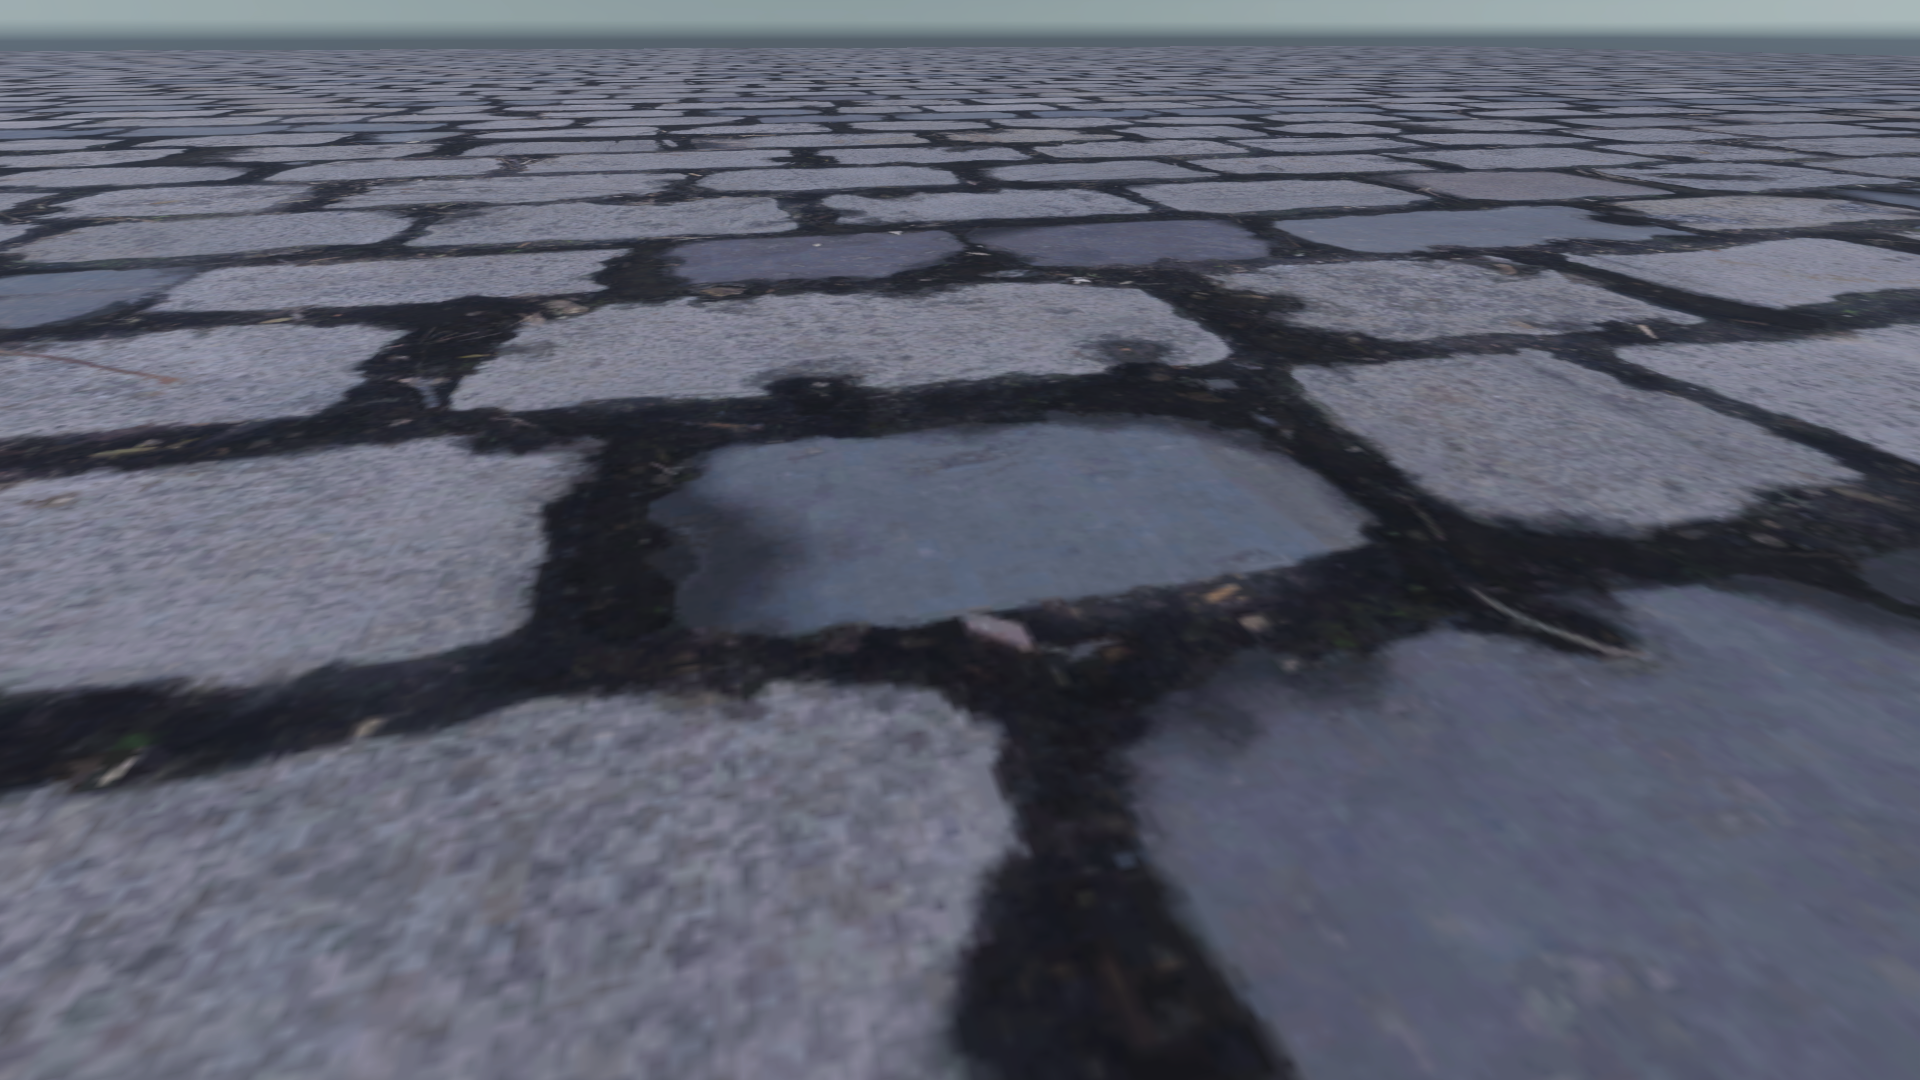
\includegraphics[width=0.49\textwidth]{Grafiken/Basics/Mapping/Vergleich_Diffuse.png}
	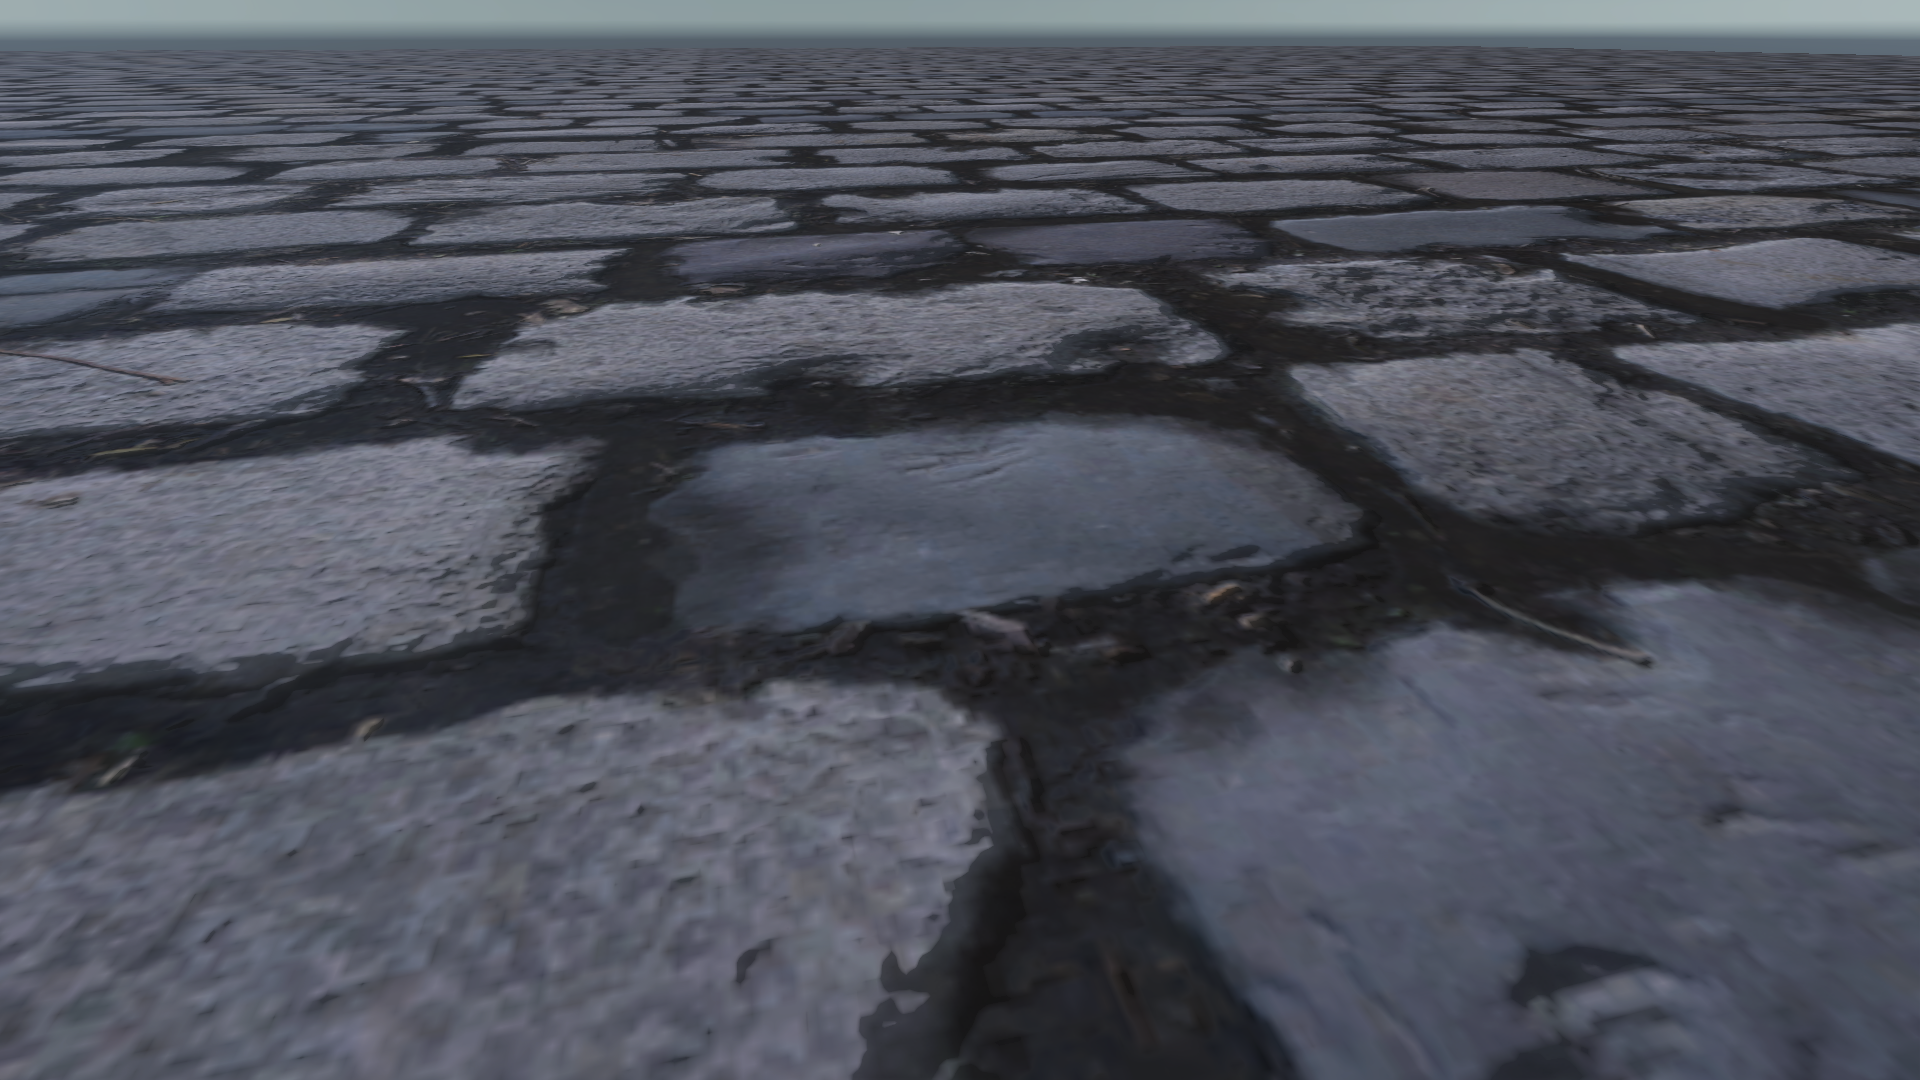
\includegraphics[width=0.49\textwidth]{Grafiken/Basics/Mapping/Vergleich_Normal.png}
	\begin{footnotesize}
		\caption{links: Einfache diffuse Beleuchtung der Textur, rechts: Normal Mapping. Beide Geometrien sind komplett flach. 
		Hierbei sieht man gut den Unterschied zwischen dem flachen Look
		der diffus beleuchteten Textur und dem realistischeren Aussehen durch Einbeziehen der Oberflächennormalen aus der Normal Map.}
	\end{footnotesize}
\end{figure}

\subsubsection{Displacement Mapping}
Mit Displacement Mapping werden dagegen tatsächlich, mithilfe von Heightmaps, die Positionen
der Vertices entlang ihrer Normalen versetzt \parencite{Cook1984,Cook1987}. Dadurch kommt es nicht zu blickwinkelabhängigen Artefakten
und die Illusion von Tiefe wird real. Objekte sehen aus einem flachen Winkel betrachtet nicht mehr
glatt aus, sondern haben tatsächlich Struktur in ihrer Oberfläche. Damit dieser Effekt jedoch zustande kommt,
muss das Mesh in einer gewissen Auflösung zur Verfügung stehen. Je nach Detailreichtum der Heightmap
muss die Geometrie dabei in weitere Polygone unterteilt werden. Der Vorteil hierbei ist der hohe
Grad an Realismus. Ein deutlicher Nachteil liegt dabei allerdings in der Performance.
Ein weitgehender Einsatz von Displacement Mapping kann eine hohe Polygonanzahl schnell
negativen Einfluss auf die Renderingzeiten nehmen. 


\subsubsection{Parallax Mapping}

Parallax Mapping (oder auch Offset (Bump-)Mapping) ist eine weitere Methode, um sich die Möglichkeiten von
Bump Mapping-Verfahren zunutze zu machen. Anders als bei tatsächlicher Modifizierung der Vertices
durch Displacement Maps werden hier nur die Texturkoordinaten abhängig vom Blickwinkel verschoben. \parencite{Kaneko2001, Welsh2004}
Durch Bewegung der Oberfläche oder des Betrachters entsteht somit ein realistischerer Eindruck
von Tiefe in der Textur, welcher den des Displacement Mappings approximiert darstellt.
Dabei ist Parallax Mapping allerdings immer noch deutlich effizienter als echtes Vertex-Displacement
und eignet sich daher eher für Echtzeitrenderings.
Parallax Mapping alleine simuliert zwar den Parallax-Effekt, jedoch ist es hiermit nicht möglich, die Silhoutte zu verändern und
Selbstschattierung oder -verdeckung vorzutäuschen.


\subsubsection{Parallax Occlusion Mapping}
\label{sec:3.3.4}

\begin{figure}[h]
	\centering
	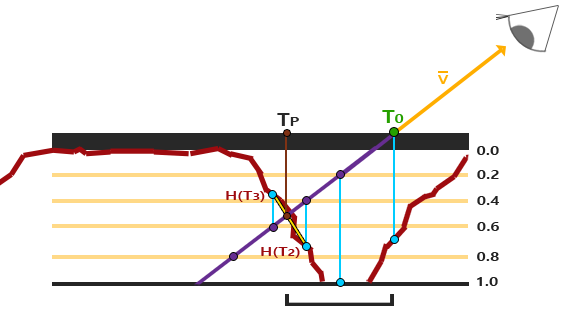
\includegraphics[width=0.8\textwidth]{Grafiken/Basics/Mapping/Infografik_POM.png}
	\begin{footnotesize}
		\caption{Verschiebung der Texturkoordinaten beim Parllax Occlusion Mapping}
	\end{footnotesize}
\end{figure}


Parallax Occlusion Mapping (POM) ist eine komplexere, verbesserte Variante des Parallax Mapping, basierend auf einem Per-Pixel Ray Tracing.
Das Ziel ist auch hier wieder das Vorherige: Detaillierte Oberflächen ohne den Preis von teuren Vertexverschiebungen.
Diese Details lassen sich abhängig vom Blickwinkel aus jeder Perspektive korrekt darstellen.
Durch Einsatz von dynamischer Beleuchtung und Selbstokklusion kann außerdem eine korrekte Selbstschattierung simuliert werden \parencite{Brawley2004, Tatarchuk2006}.
Die Informationen aus der Heightmap werden hierbei für Berechnungen im Fragmentshader verwendet.
Anstatt wie beim Displacement Mapping Details zu extrudieren, wird bei POM in die Tiefe simuliert.
Hierbei wird für die Oberfläche der Wert 1.0, und damit der höchste Punkt, angenommen.
Zunächst wird für jeden zu rendernden Pixel mittels Ray Castings vom Betrachter zur Geometrie-Oberfläche ein Schnittpunkt  $T_0$ ausfindig gemacht.
Der Strahl $\vec{v}$ wird nun weiter durch das – durch die Heightmap ausgedrückte – Volumen verfolgt und Schrittweise abgetastet. Wenn sich der Strahl 
mit der Heightmap im Punkt $T_P$ schneidet, kann mit der Position die neue, zu rendernde Texturkoordinate ermittelt werden. 
Je geringer die Schrittweite ist, desto genauer kann die Oberfläche gerendert werden.
Ist die Schrittgröße zu groß, kann die Heightmap nicht detailliert genug abgetastet werden und es entstehen Aliaseffekte. Es zeichnet sich
ein Treppeneffekt ab (\autoref{fig:alias}). Zusätzlich kann ein zu starkes Offset die Textur unnatürlich weit verzerren. 


\begin{figure}[ht]
	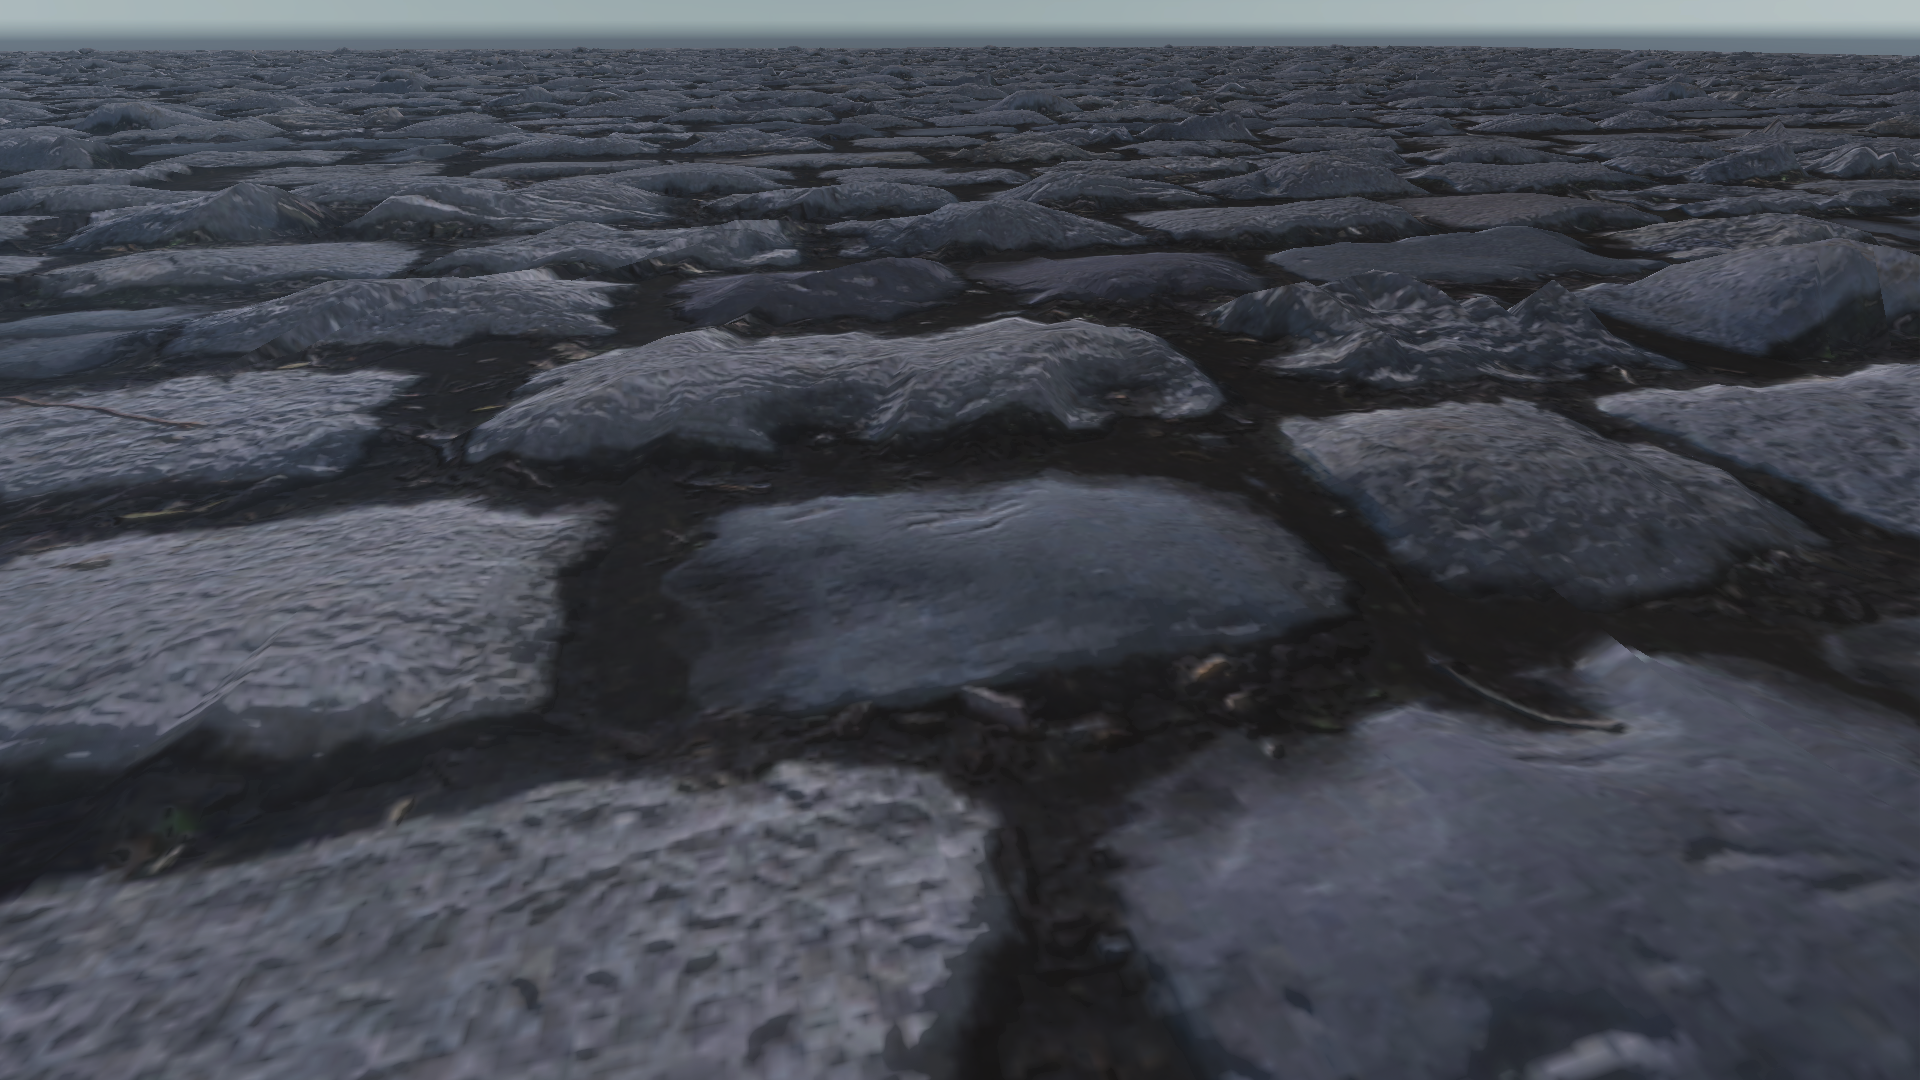
\includegraphics[width=0.49\textwidth]{Grafiken/Basics/Mapping/Vergleich_DisplacementNormalTesselated.png}
	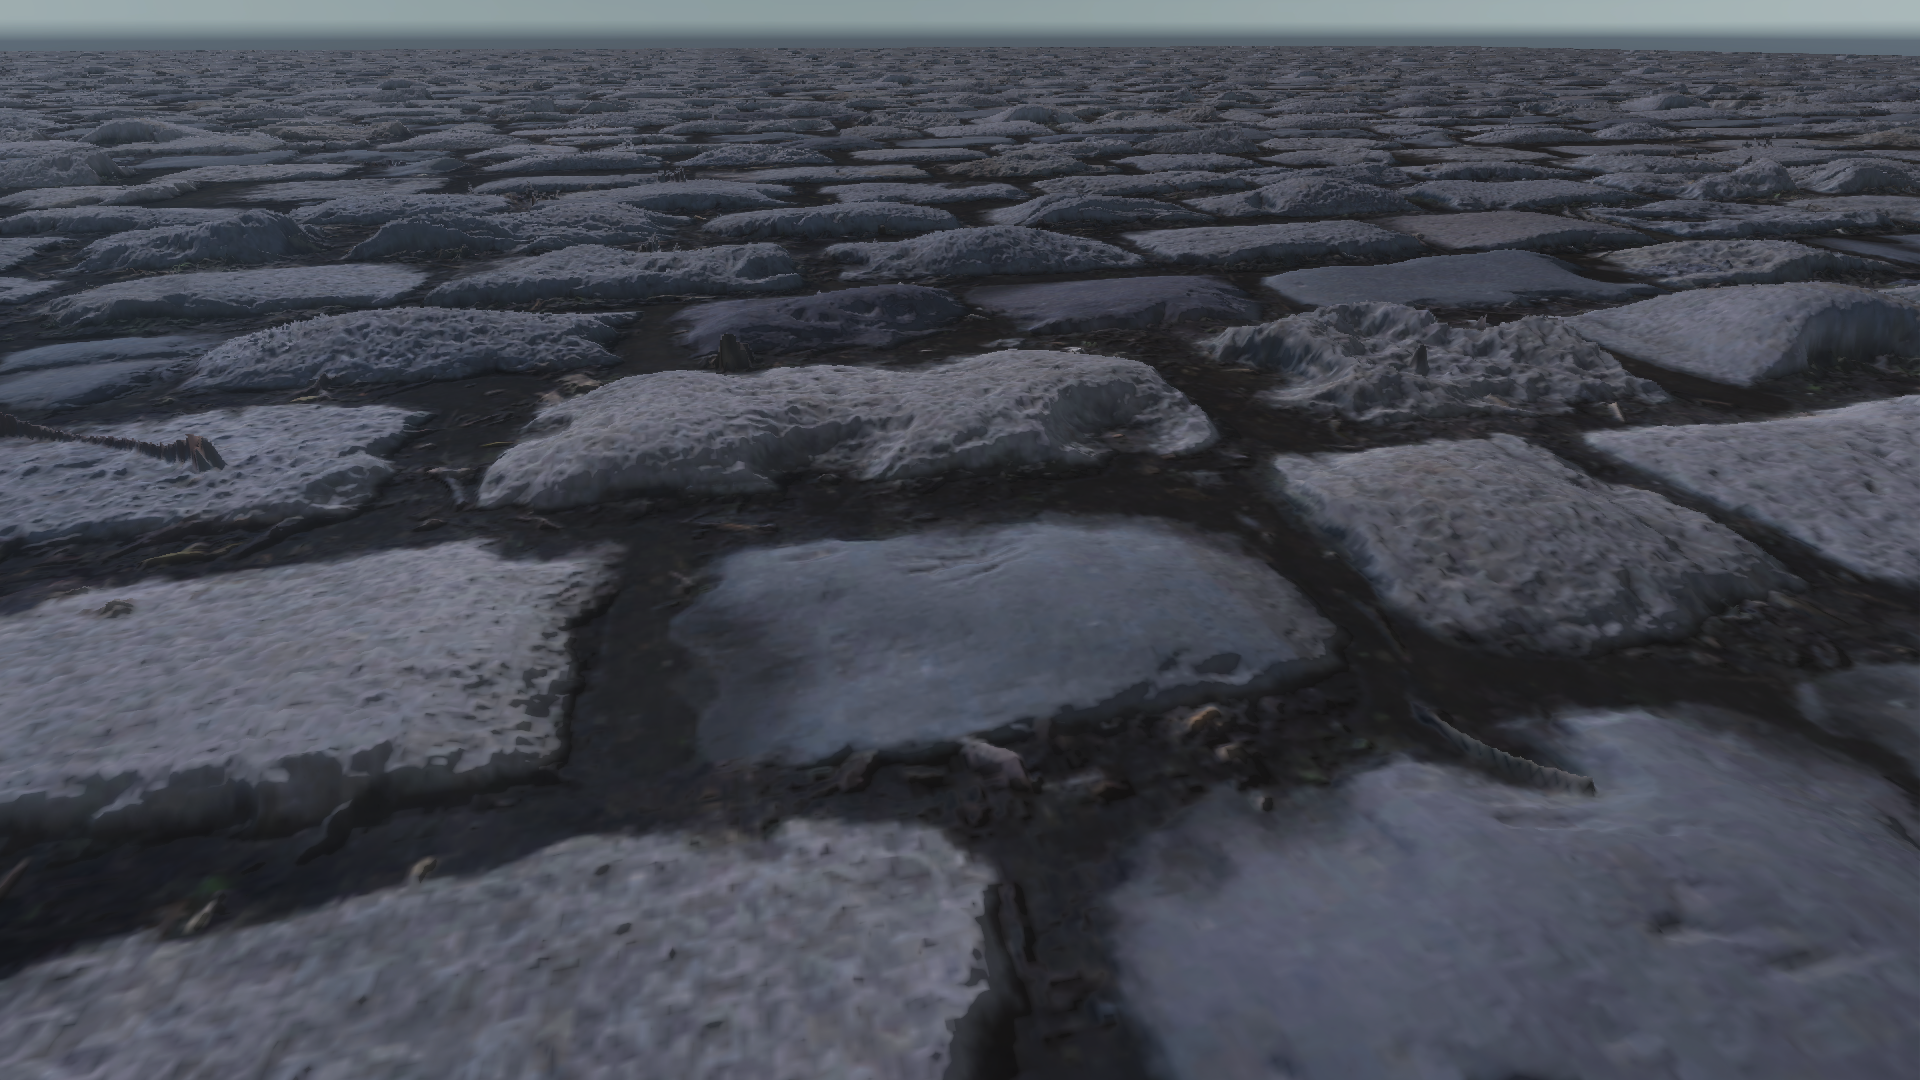
\includegraphics[width=0.49\textwidth]{Grafiken/Basics/Mapping/Vergleich_POM_64Steps.png}
	\begin{footnotesize}
		\caption{links: Displacement Map, Normal Map und 50-facher Tesselation, rechts: Parallax Occlusion Mapping mit 64 Samples. 
		Beide Methoden sehen sich sehr ähnlich, der Unterschied ist jedoch, dass für die Displacement Map-Methode in diesem Beispiel die 50-fache Anzahl an
		Dreiecken gebraucht wird.}
	\end{footnotesize}
\end{figure}


\begin{figure}[h]
	\centering
	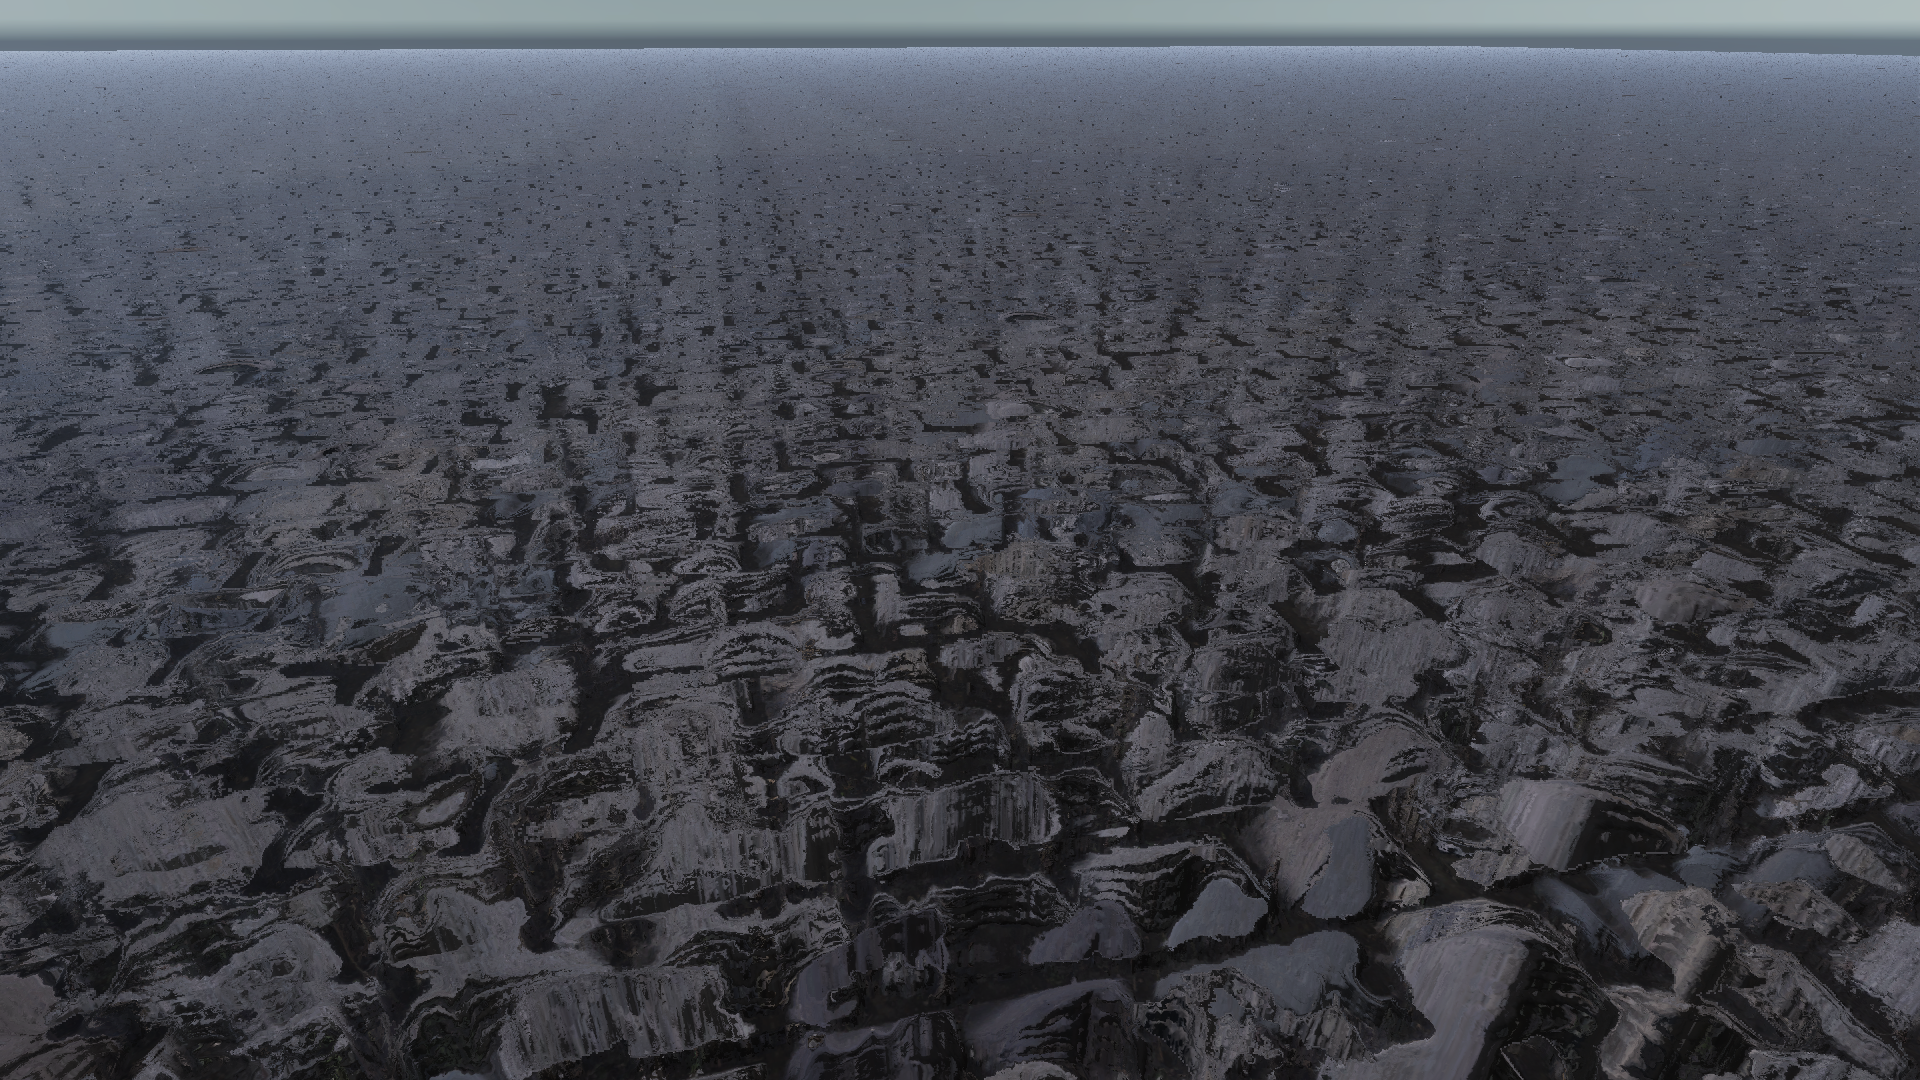
\includegraphics[width=1\textwidth]{Grafiken/Basics/Mapping/aliasing.png}
	\begin{footnotesize}
		\caption{Aliasingeffekt bei zu geringer Sampleanzahl mit 4 Schritten.}
		\label{fig:alias}
	\end{footnotesize}
\end{figure}


\subsection{Volume Rendering}
\subsubsection{Ray-Marching}
\subsubsection{Texturbasierte Volumen}


\newpage

\section{Konzeption und Umsetzung}
\label{sec:4}
\subsection{Entwurf}

Da die Ergebnisse dieser Arbeit relevant für das KoViTReK Forschungsprojekt\footnote{https://www.th-koeln.de/anlagen-energie-und-maschinensysteme/kovitrek_87259.php} 
sein könnten und dieses in der Laufzeit- und Entwicklungsumgebung Unity\footnote{https://unity.com} 
implementiert werden soll, werden auch die Partikelsysteme in der selben Software entworfen. 

Werden die Texturen Prozedural als Shader erstellt? 
-> POM müsste möglicherweise mit Blender/Houdini/Flipbooks erstellt werden, man könnte 6wayLightmapping einbauen
-> Raymarching kann man Prozedural generieren, da random Volume benötigt wird.



\subsection{Erstellung der Texturen}

\subsubsection{Texture Sheets}

Die Texturen werden auf zwei verschiedene Arten erstellt. Für die Variante mit Parallax Occlusion Mapping werden \textcolor{red}{zwei/drei} 
Texturen in \textcolor{red}{Blender/HOUDINI} erstellt. Hier lassen sich relativ einfach und schnell visuell überzeugende Rauch- und 
Feuersimulationen erstellen. Die Simulationen basieren auf Fluidberechnungen, wodurch ein realistisches Abbild erzeugt werden kann. 
Die Animation wird daraufhin in einzelnen Frames auf einer Textur in einem Grid abgespeichert, auch Sprite Sheet oder Flipbook genannt.
Jeder Frame wird in der Textur mit einer Auflösung von 128 x 128 px gespeichert. Bei einer Frameanzahl von 8x8 = 64 Frames entspricht das also
einer Auflösung der ganzen Textur von 1024 x 1024 px.
In jedem Frame werden in Textur 1 die Tangent-Lightmaps (Top/Left/Right) in den jeweiligen RGB-Channels gespeichert. 
Der Alpha-Channel enthält die Bottom-Lightmap. In Textur 2 wird eine Heat-/Emissionmap im Rot-Channel gespeichert, die Alphainformation im 
Grün-Channel und die für das Parallax-Occlusion-Mapping benötigte Heightmap im blauen Farbkanal. Der Alpha-Channel wird hierbei nicht benutzt.
In den beiden Texturen fehlen nun noch die Beleuchtung aus den Richtungen von Vorne und von Hinten. Diese werden allerdings im Shader 
berechnet, anstatt sie in die Textur zu backen. Aus den verschiedenen Lightmaps kann daraufhin basierend auf der Richtung des Lichteinfalls 
auf die Textur relativ günstig und performant eine korrekte Beleuchtung des Rauchs generiert werden. 



\subsection{Shader}
Für das Rendering der Partikel werden zwei Shader entwickelt. Diese basieren auf Parallax Occlusion 
Mapping und auf Raymarching durch eine Volumentextur. 

\subsubsection{Parallax Occlusion Mapping}

\subsubsection{Raymarcher}

\subsection{Partikelsystem}
Um die Partikelsysteme umzusetzen wird der relativ junge, von Unity entwickelte Editor 'Visual Effects Graph' 
(kurz: VFX Graph) verwendet. VFX Graph ist ein nodesbasierter Editor, um schnell
dynamische und komplexe Partikelsysteme zu erzeugen\footnote{https://unity.com/de/visual-effect-graph}.
Im Gegensatz zum älteren Shuriken-Partikelsystem von Unity werden die Partikel hier auf der GPU
simuliert, wodurch das System deutlich an Performance gewinnt und ein mehr Partikel zeichnen kann. 
Shuriken nimmt die Berechnungen im Gegensatz zum VFX Graph auf der CPU vor\footnote{https://docs.unity3d.com/Manual/ChoosingYourParticleSystem.html}. 
Gerade für VR-Anwendungen bietet sich also dieses neue System an.
VFX-Graph hat jedoch nur sehr begrenzte Möglichkeiten, was Physiksimulationen und Kollisionen der Partikel angeht. 
Es muss also ein System erstellt werden, welches trotz der Einschränkungen ein möglichst realistisches 
Verhalten der Feuer- und Rauchpartikel gewährleistet.  




\newpage

\section{Evaluierung der Methoden}
\label{sec:5}
\markboth{Evaluierung der Methoden}{Evaluierung der Methoden}

Beide Methoden haben ihre Vor- und Nachteile. Die realistische Darstellung von voluminösen Materialien verlangt
eine besondere Herangehensweise, welche sich – im Gegensatz zu undurchsichtigen, festen Oberflächen –
nicht überzeugend mit herkömmlichen Texture-Mapping Methoden umsetzen lässt.
Die Implementierung der Systeme ist aufgrund der begrenzten Zeit im Rahmen dieser Arbeit nur prototypisch mithilfe der
zur Verfügung stehenden Funktionen aus Unity implementiert und daher nicht bestmöglich optimiert.
In \textbf{\autoref{sec:6.3}} werden einige Optimierungsmöglichkeiten präsentiert.
Die Vor- und Nachteile, sowie das Potential für den Nutzen der jeweiligen Methoden lassen sich dennoch aus dem Entwurf
herausarbeiten und werden in den folgenden Abschnitten beschrieben.


\subsection{Parallax Occlusion Mapping}
\label{sec:5.1}


POM ist eine komplexere Variante des Normalmappings. Dementsprechend ist auch POM eine Technik für feste Oberflächen und weniger
für den Einsatz bei der Simulation von Volumen gedacht. Um aber die Effizienz der Billboard-basierten Partikelsysteme
nutzen zu können ist das Parallax Occlusion Mapping eine interessante Möglichkeit, die es wert ist, getestet zu werden.
Trotz der erhöhten Komplexität des Algorithmus gegenüber klassischeren Mappingverfahren läuft die Anwendung auf dem Testsystem
stabil mit 90FPS. Hier gibt es also keine Bedenken hinsichtlich der Shaderperformance. Auch die aufwändige Berechnung der
Fluidsimulationen wird hier im Voraus erledigt. Somit ist es möglich, realistisch aussehende Partikelsysteme unter geringem
Rechenaufwand in der Echtzeitanwendung zu erzeugen und diese dabei noch realistisch aussehen zu lassen.
Ein weiterer Vorteil, der sich aus der Natur des schwarzen Rauches bei Bränden ergibt, ist die Tatsache, dass die genaue Berechnung
von Selbstschattierungen hierbei nicht so essentiell ist wie bei weißem Rauch.
Dies ist zwar nicht direkt ein Vorteil von POM, gleicht aber einen Nachteil aus, den es in der Anwendung in einem Partikelsystem gibt.
Die Texturen auf den Billboards sind in der Lage, sich individuell selbst zu schattieren, gegenseitig ist dies jedoch nicht möglich \autoref{fig:pomShadows}. 
In Bezug auf den Schatten generell gibt es das Problem, dass Billboard-basierte Partikelsysteme eigentlich nur flache Sprites sind und deshalb nicht in der 
Lage sind, realistische Schatten auf die Umgebung werfen zu können. In Hinblick auf die Beleuchtung ist es mit POM auch möglich, eine geringe Anzahl dynamischer 
Lichtquellen einzubeziehen (\autoref{fig:dynamicLightingSmoke}).

\begin{figure}[h!]
	\centering
	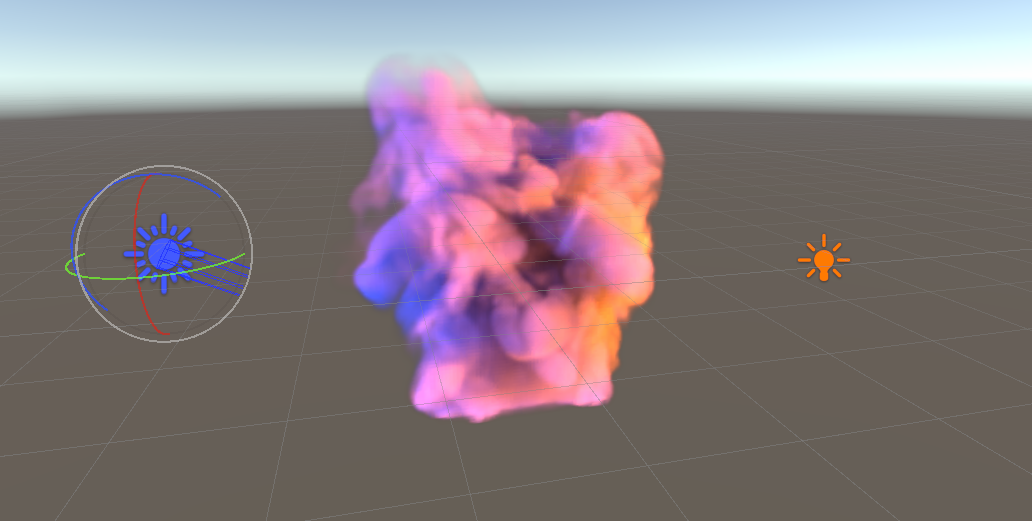
\includegraphics[width=0.89\textwidth]{Grafiken/Implementation/litSmoke.png}
	\begin{footnotesize}
		\caption{Dynamische Beleuchtung des Rauchs}
		\label{fig:dynamicLightingSmoke}
	\end{footnotesize}
\end{figure}



\begin{figure}[h!]
	\centering
	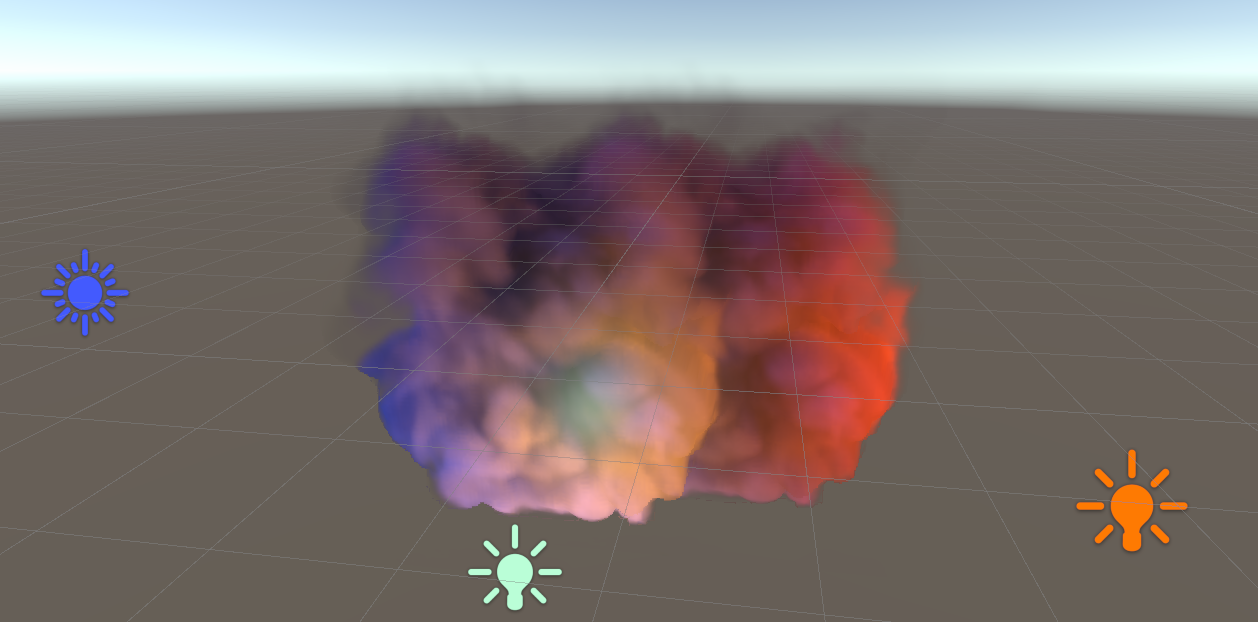
\includegraphics[width=0.89\textwidth]{Grafiken/Evaluation/pomShadows.png}
	\begin{footnotesize}
		\caption{Kein gegenseitiger Schattenwurf bei POM-basierten Billboards. }
		\label{fig:pomShadows}
	\end{footnotesize}
\end{figure}




%How, wie viele?

Ein weiterer Vorteil, der sich aus dieser Methode ergibt, sind die Texture Sheets. In eine einzige Textur lassen sich 4 verschiedene Informationen in die
RGBA-Kanäle speichern. Neben den verschiedenen Lightmaps aus 6 Richtungen können beispielsweise noch ein Color-Key oder Emission- und Heatmaps gespeichert werden.
Mit weiteren Infos wie einer Heatmap lässt sich ein Übergang, bzw. eine Mischung von Feuer und Rauch erzeugen. Dies ist ein Phänomen, welches sich bei größeren Bränden
oder Explosionen beobachten lässt (\autoref{fig:explosion}).
Die Anzahl der Lightmaps lässt sich auch reduzieren, indem die Lichtrichtungen von vorne und von hinten im Shader approximiert werden können.
Es gibt viele Möglichkeiten, die Flexibilität von Texturen ausnutzen zu können und dabei die Menge an benötigten Daten und Berechnungen gering zu halten,
sodass der flüssige Einsatz in VR gegeben bleibt. Weiterhin lassen sich auf Kosten weiterer Texture Sheets
verschiedene Simulationen erstellen, sodass größere Varianz in das Aussehen des Partikelsystems eingebracht werden kann.
Durch die unendliche Wiederholbarkeit kann die Animation ab einem zufällig gewählten Frame starten, wodurch schon mit einer einzigen Animation
kaum auffällt, dass das ganze System auf dieser einen Animation basiert.


Neben den ganzen Vorteilen, die diese Variante mit sich bringt gibt es auch negative Punkte. Bei zu geringer Auflösung sehen die Renderings schnell
verpixelt aus, je näher diese betrachtet werden. Dies ist ein großer Nachteil der Texture Sheets. Wird die Auflösung jedes Frames verdoppelt, also in diesem
Fall von 256x256 Pixeln auf 512x512 Pixel, so erhöht sich die Auflösung der gesamten Textur um den Faktor vier für jeden der RGBA-Kanäle. Selbst dann sind
die einzelnen Frames noch relativ gering aufgelöst und nicht für die Betrachtung aus der Nähe gedacht. Je detaillierter die Simulation auf denen die Texture Sheets basieren,
desto höher sollte die Auflösung sein um auch alle diese Details abbilden zu können.
Die visuellen Artefakte, wie beispielsweise das Einschneiden der benachbarten Frames aus dem Texture Sheet aus einem flachen Betrachtungswinkel (\autoref{fig:smokeBleeding}),
schränken die Einsatzmöglichkeiten für die Anwendung in VR stark ein.
Bei der Darstellung des Feuers kommt der Faktor hinzu, dass Billboards nicht als Lichtquelle fungieren, was dem Realismus der Simulation schadet.

Abschließend lässt sich zu dem Rendering von Feuer und Rauch auf Basis von Parallax Occlusion Mapping sagen, dass sich diese Variante, so wie sie für diese Arbet
implementiert ist, nicht immer eignet. Die visuellen Artefakte erzeugen Störungen der Immersion. Jedoch wird das Parallax Offset in der Stereoansicht korrekt dargestellt,
wodurch dieser Ansatz vielversprechend bleibt. Es ist wahrscheinlich, dass es für die genannten Probleme elegante Lösungen gibt, die in Zukunft an anderer Stelle 
betrachtet werden könnten.



CONTRA\newline
- Transparenz ist irgendwie weird\newline
- Geringe Auflösung der einzelnen Frames, doppelte Auflösung = 4fache Texturgröße \newline
% - Basiert immernoch auf Billboards\newline
%  -> Trotz simulierter Tiefe ein flacher Eindruck in VR\newline
- Funktioniert nicht gut bei mehreren Lichtquellen\newline
- Schattenwurf auf Umgebung funktioniert nicht\newline
- Beleuchtung der  Umgebung auch nicht möglich\newline

\begin{figure}[h!]
	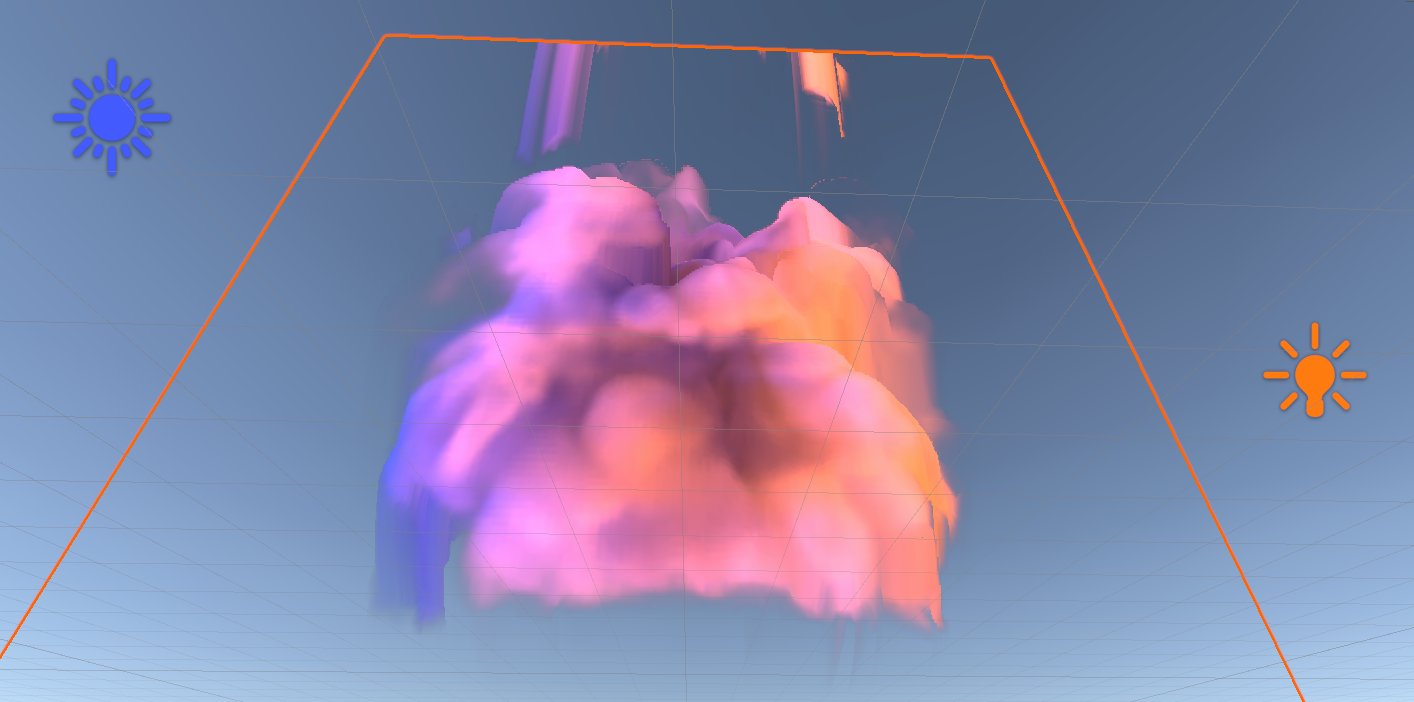
\includegraphics[width=0.89\textwidth]{Grafiken/Evaluation/Smoke_artefacts.png}
	\centering
	\begin{footnotesize}
		\caption{Verzerrungsartefakte bei der Anwendung von Parallax Occlusion Mapping mit zu starkem Offset. Die benachbarten Frames des Texture Sheets
			werden ebenfalls mit verzerrt, wodurch Fragmente davon, bei flachem Betrachtungswinkel, mit in das Billboard einlaufen.}
		\label{fig:smokeBleeding}
	\end{footnotesize}
\end{figure}



\subsection{Ray Marching}
\label{sec:5.2}

PRO: \newline
- Sehr günstige AO aufgrund der bereits berechneten Distanz\newline
- Lichtstrahl in Volumen weiterverfolgen kann Schatten erzeugen\newline
-

CONTRA: \newline
- Aufwändigere Berechnung\newline
- 3D-Datenset beinhaltet keine Animation der Textur\newline





\section{Ergebnisse}
\label{sec:6}
Hier kommen die Erkenntnisse meiner Arbeit rein
\subsection{Zusammenfassung}
\label{sec:6.1}



\subsection{Limitationen}
\label{sec:6.2}
\subsection{Ausblick}
\label{sec:6.3}

\newpage





%%%%%%%%%%%%%%%%%%%%%%%%%%%%%%%
%%%%%%%%%% LITERATUR %%%%%%%%%%
%%%%%%%%%%%%%%%%%%%%%%%%%%%%%%%
\newpage
\begin{thebibliography}{1}\markboth{Literaturverzeichnis}{Literaturverzeichnis}\addcontentsline{toc}{section}{Literaturverzeichnis}
	
	\bibitem{AV}
	Volker, Ahrens: 
	Abschlussarbeiten richtig gliedern in Naturwissenschaften, Technik und Wirtschaft,
	Zürich: vdf, 
	2014.
	
	\bibitem{BM}
	Bechtel, Michael; Thomas, Volker:
	Schreiben über Technik,
	Konstanz: UVK,
	2011.
	
\end{thebibliography}
\newpage
\newpage



%%%%%%%%%%%%%%%%%%%%%%%%%%%%%%%
%%%%%%%%%% ERKLÄRUNG %%%%%%%%%%
%%%%%%%%%%%%%%%%%%%%%%%%%%%%%%%
\section*{Eidesstattliche Erklärung}
% \addcontentsline{toc}{section}{Eidesstattliche Erklärung}
Ich erkläre an Eides statt, dass ich die vorgelegte Abschlussarbeit selbständig und ohne fremde Hilfe verfasst, andere als die angegebenen Quellen und Hilfsmittel nicht benutzt und die den benutzten Quellen wörtlich oder inhaltlich entnommenen Stellen als solche kenntlich gemacht habe.
~\\
~\\
\rule{0.35\textwidth}{0.4pt} \hspace*{3cm} \rule{0.45\textwidth}{0.4pt} \newline
Ort, Datum	\hspace*{6.3cm}	Rechtsverbindliche Unterschrift

%%%%%%%%%%%%%%%%%%%%%%%%%%%%%%%
%%%%%%%%%%   ENDE    %%%%%%%%%%
%%%%%%%%%%%%%%%%%%%%%%%%%%%%%%%
\newpage
\pagestyle{empty}
\begin{flushleft}
	TH Köln \newline
	Gustav-Heinemann-Ufer 54\newline
	50968 Köln\newline
	www.th-koeln.de\newline
\end{flushleft}

\begin{figure}[b]
	\begin{flushright}
		
\includegraphics[scale=1]{Grafiken/TH/TH_LOGO}\\
	\end{flushright}
\end{figure}


\end{document}